\documentclass{article}



\usepackage{arxiv}

\usepackage[utf8]{inputenc} % allow utf-8 input
\usepackage[T1]{fontenc}    % use 8-bit T1 fonts
\usepackage{hyperref}       % hyperlinks
\usepackage{url}            % simple URL typesetting
\usepackage{booktabs}       % professional-quality tables
\usepackage{amsfonts}       % blackboard math symbols
\usepackage{nicefrac}       % compact symbols for 1/2, etc.
\usepackage{microtype}      % microtypography
\usepackage{graphicx}
\usepackage{natbib}
\usepackage{amsmath}
\usepackage[ruled,linesnumbered]{algorithm2e}
\usepackage{microtype}
\usepackage{float}
\usepackage{listings}
\usepackage{subcaption}
\usepackage{enumitem}
\usepackage{doi}



\title{Selection of output mode for Bayesianoptimization in noisy problems}

%\date{September 9, 1985}	% Here you can change the date presented in the paper title
%\date{} 					% Or removing it

\author{ \href{https://orcid.org/0000-0000-0000-0000}{
\includegraphics[scale=0.06]{orcid.pdf}\hspace{1mm}Chenxi Li}\thanks{Use footnote for providing further
		information about author (webpage, alternative
		address)---\emph{not} for acknowledging funding agencies.} \\
	Department of Information Systems and Management Engineering\\
	Southern University of Science and Technology\\
	Shenzhen, China\\
	\texttt{12333226@mail.sustech.edu.cn} \\
	%% examples of more authors
	%% \AND
	%% Coauthor \\
	%% Affiliation \\
	%% Address \\
	%% \texttt{email} \\
	%% \And
	%% Coauthor \\
	%% Affiliation \\
	%% Address \\
	%% \texttt{email} \\
	%% \And
	%% Coauthor \\
	%% Affiliation \\
	%% Address \\
	%% \texttt{email} \\
}

% Uncomment to remove the date
%\date{}

% Uncomment to override  the `A preprint' in the header
%\renewcommand{\headeright}{Technical Report}
%\renewcommand{\undertitle}{Technical Report}
\renewcommand{\shorttitle}{\textit{arXiv} Template}

%%% Add PDF metadata to help others organize their library
%%% Once the PDF is generated, you can check the metadata with
%%% $ pdfinfo template.pdf
\hypersetup{
pdftitle={A template for the arxiv style},
pdfsubject={q-bio.NC, q-bio.QM},
pdfauthor={David S.~Hippocampus, Elias D.~Striatum},
pdfkeywords={First keyword, Second keyword, More},
}

\begin{document}
\maketitle

\begin{abstract}
	\hspace{2em}This paper explores the method of Bayesian optimization for selecting the final output result in noisy optimization problems. For noise-free problems, the best observation can be directly output as the final optimization result. However, in the presence of noise, each observation is affected by the noise and it may not be appropriate to output the best observation directly. Considering that the surrogate models in Bayesian optimization are able to provide predicted mean for any point in the search space, and for noisy objective function, the predictions of the model tend to be more plausible than the actual observations. This inspired us to use a result output method based on the predicted values of thesurrogate models. For example, assuming that we want to find the minimum of the objective function, we can output the point with the lowest predicted mean among all observed points, or the point with the lowest predicted mean in the entire search space. In the case of high noise levels, these methods may be more appropriate than using the observations directly. However, the choice of output method depends not only on the noise level, but may also depend on factors such as the response surface properties and the dimensionality of the search space. In this paper, we will conduct numerical experiments using the BBOB function set to investigate the advantages and disadvantages of each output method for Bayesian optimization in different noise environments, and provide informative suggestions for the choice of output methods.

\end{abstract}


% keywords can be removed

\keywords{Bayesian optimization \and Gaussian process \and blackbox optimization \and noisy problems \and BBOB}


\section{Introduction}

\hspace{2em}
Bayesian optimization stands out as an advanced optimization framework for  black-box optimization. The advantage of this method is the ability to approximate the global optimum with fewer objective functions to evaluate. This efficiency makes it a widely adopted approach in diverse domains, including drug research and development, as well as cost-effective optimization challenges such as the adjustment of neural network parameters and other objective function evaluations \citep{Shahriari2016taking}.The algorithm is a model-based sequential optimization. At each iteration, Bayesian optimization will formulate a strategy that balances exploration and development based on the currently available information to select the next evaluation point. In particular, Bayesian optimization is primarily made up of two parts: the surrogate model and the acquisition function. The surrogate model generally uses Gaussian process \citep{Rasmussen2005Gaussian} for simulating the objective function based on current observation points. The acquisition function can then use the established model to select the location of the next observation point, thereby optimizing outcomes more efficiently with fewer observations.

\hspace{2em}
Bayesian optimization demonstrates its efficiency in many scenarios, especially in low-dimensional, noise-free and expensive black-box optimization problems. When the objective function is noisy, Bayesian optimization faces a critical problem in that the observations corresponding to the observation points are no longer accurate. This problem may affect the effectiveness of Bayesian optimization in two ways: the acquisition function and the output results. Presently the most commonly used acquisition function is EI \citep{Jones1998Efficient} which based on the optimal value improvement expectation. That is, by calculating the expected improvement of a specific point relative to the current optimal value, the point with the largest expectation improvement is selected as the next observation point. In cases of high noise level, the current optimal value may be seriously disturbed, thus affecting the point selection strategy of EI, making it tend to over-explore. Smilarly, noise level also affects our final output results, as the minimum observation in this case is also not accurate. An intuitive solution to these problems is to replace the observed optimum with the optimum of the predicted mean derived by the agent model. Here the predicted mean is the agent model's extrapolation of the objective function based on the available information. In noisy situations, these predictions are often more reliable than direct observations. The main purpose of the research in this paper is to explore the circumstances under which we should trust predicted values more than observed values. To the best of our knowledge, this does not seem to have been discussed in detail in current articles, so this paper attempts to explore it through numerical experiments. In order to make the experimental conclusions more representative, the test problemss in this paper choose to use the advanced test benchmark environment "BBOB",  inclusive of 24 noise-free test functions. We modified it to be in a noisy form as a benchmark question for the numerical experiments. The detail of BBOB functions can be found in \citep{Hansen2010RealParameterBO}

\hspace{2em}
The structure of this article is segmented as follows: The first part is a detailed introduction to Bayesian optimization, includeing surrogate model and acquisition function. The second part is an introduction to BBOB benchmark functions and experimental settings. In the third part, we discussed the use of observations and predictions in a noise-free environment value as the difference in optimization effect as the result output. The fourth part is a noisy experiment. 


\section{Bayesian optimization}
\hspace{2em}Assume f (x) is an unknown target black-box function, Consider the optimization problem:
\begin{equation}\label{eq1}
	x^* = \mathop{\arg\max}\limits_{x \in \mathcal{X}} f(x)
\end{equation}
where X is the disign space assumed compact. The objective function f(x) has no explicit expression, for any $x_0 \in \mathcal{X}$(observation point), the corresponding objective function value $f(x_0)$ can be calculated(observation value).Bayesian optimization frameworks commonly employ Gaussian processes (see Section 2.1) as surrogate models to construct the posterior distribution of the objective function, providing a high degree of flexibility. With Gaussian process modeling, the model can yield the predicted mean and uncertainty for any point in the search space. Leveraging these predicted values and uncertainties, we can design acquisition functions (see Section 2.2) to balance exploration and exploitation, thereby selecting the next observation point. The specific algorithm of Bayesian optimization is outlined in \textbf{Algorithm1}.

\hspace{2em}
Note that \textbf{Algorithm1} provides the standard Bayesian optimization algorithm under the assumption of a noise-free condition. In the presence of noise, outputting the point corresponding to the minimum observed value as the result may not be appropriate. Two alternative predictive output methods may be considered: outputting the point with the smallest predicted mean among the observation points or outputting the point with the smallest predicted mean throughout the entire design space as predicted by the surrogate model. The following experimental segment will focus on examining and contrasting the optimization efficacy of these output methods.
\begin{algorithm}[htb]
    \SetAlgoLined
    \KwIn{number of initial point $n_0$,\ number of max iteration $n$}
  
    Randomly get initial data $D_{1:n_0}$ and update GP model\;
    \For{$t=1,2,...n$}{
     Find $x_t$ by optimizing the acquisition function over the GP $x_t={\arg\max}_x u(x|D_{1:n_0+n})$\;
     Sample the objective function: $y_t=f(x_t)+\epsilon_t$\;
     Augment the data $D_{1:n_0+n}$ = ${D_{1:n_0+n-1},(x_t,y_t)}$ and update GP model\;
     }
    \KwResult{$(x_{t^*},y_{t^*}) \in D_{1:n_0+n}$,\ $t^*=\mathop{\arg\max}y_{1:n_0+n}$}
    \caption{Bayesian optimization}
\end{algorithm}






\subsection{Gaussian process}
\hspace{2em}Gaussian process is a nonparametric model that is fully characterized by its prior mean function $m(x):\mathcal{X} \rightarrow \mathbb{R}$ and positive definite kernel functions(Can also be thought of as a covariance function) $k:\mathcal{X} \times \mathcal{X} \rightarrow \mathbb{R}$. For any finite set of points within the search space $x_{1:n}$, define $f_i:=f(x_i)$ as the corresponding value of the objective function at $x_i$, $y_i:=f(x_i)+\epsilon_i$ is the corresponding noisy observation at $x_i$.In the Gaussian process model, we assume that $\textbf{f}:=f_{1:n}$ obeys a joint Gaussian distribution, and that $\textbf{y}:=y_{1:n}$ obeys a normal distribution given $\textbf{f}$, which is expressed as follows:
\begin{equation}\label{eq2}
    \textbf{f}\mid\mathcal{X} \sim \mathcal{N}(\textbf{m},\textbf{K})
    \end{equation}
    \begin{equation}\label{eq3}
    \textbf{y}\mid \textbf{f},\sigma^2 \sim \mathcal{N}(\textbf{f},\sigma^2\textbf{I}])
    \end{equation}
Note here we treat the objective function $f(x)$ as a random variable, and equation(2) represents the prior distribution of the variable $f(x)$. where $\textbf{m}$ represents the prior mean function, and $K_{i,j}:=k(x_i,x_j)$ is the covariance matrix. After obtaining the observation data $\mathcal{D}_n={(x_i,y_i)^n_{i=1}}$, $f(x)$ given the observed data $\mathcal{D}_n$, for the new value to be predicted $f(x^*)$, we have the following joint distribution:

\hspace*{\fill}

\qquad \qquad \qquad \quad \quad \quad \quad \quad \quad \quad \quad \quad $\begin{bmatrix} \textbf{y} \\ f(x^*) \end{bmatrix}$ $\sim$ 
$\mathcal{N}$ $\Biggl($ $\textbf{m}$,$\begin{bmatrix} \textbf{K}+\sigma^2\textbf{I} & \textbf{k} (x^*)\\ 
\textbf{k} (x^*)^T & k(x^*,x^*) \end{bmatrix}$ $\Biggl)$\\

\hspace*{\fill}

Using the conditional probability distribution formula of normal distribution, it is easy to deduce the mean and variance functions of $f(x^*)$ as follows:
\begin{equation}\label{eq4}
\textbf{m}_n(x^*)=\textbf{m}(x^*)+\textbf{k}(x^*)^T(\textbf{K}+\sigma^2\textbf{I})^{-1}(\textbf{y}-\textbf{m}(\textbf{x}))
\end{equation}
\begin{equation}\label{eq5}
\sigma^2_n(x^*)=k(\textbf{x},\textbf{x})-\textbf{k}(\textbf{x})^T(\textbf{K}+\sigma^2\textbf{I})^{-1} \textbf{k}(\textbf{x})
\end{equation}

The $\textbf{k}(x^*)$ in the formula is the vector of covariance between $x^*$ and $\textbf{x}_{1:n}$.
By employing the Gaussian process model, we can obtain the predicted mean and predicted variance for each point in the search space, which provides an important basis for the design of the acquisition function.

\subsection{Expected improvement}
\hspace{2em}BO has a variety of acquisition fuction options, including Expected improvement\citep{Jones1998Efficient}, GP upper confiddences bound\citep{Srinivas2009Gaussian}, Thompson sampling\citep{Thompson1933On}, and Entropy search methods\citep{Hennig2012Entropy}. This paper concentrates on the most commonly used method EI. The main idea of EI is to select the point with the greatest improvement expectation compared to the current optimal value as the next observation point. Specifically, we first define the improvement function $\textbf{I}$(improvement function):

\begin{equation}\label{eq6}
	\textit{I}(\textbf{x},v,\theta):=(v-f^*_n)\mathbb{I}(v>f^*_n)
\end{equation}

where $v\sim \mathcal{N}(m_n(\textbf{x}),\sigma^2(\textbf{x}))$, $\mathbb{I}$ is indicator function, $\theta$ is the hyperparameter set。
$f^*_n$ is the current optimal value, $m_n(\textbf{x}),\sigma_n(\textbf{x})$ are respectively the values returned by the Gaussian process model for the input value $\textbf{x}$ Predicted mean and predicted variance.
Take expectation for $v$ to get the acquisition function EI:

\begin{equation}\label{eq7}
	u(\textbf{x};D_{1:n}):=\mathbb{E}[\textit{I}(\textbf{x},v,\theta)]=(m_n(\textbf{x})-f^*_n)\Phi \Big(\frac{m_n(\textbf{x})-f^*_n}{\sigma(\textbf{x})}\Big)+\sigma_n(\textbf{x})\phi \Big(\frac{m_n(\textbf{x})-f^*_n}{\sigma_n(\textbf{x})} \Big)
\end{equation}

Where $\Phi$ and $\phi$ are the cumulative distribution (CDF) and probability density distribution (PDF) of the standard normal distribution respectively.

\hspace{2em}When there is noise in the objective function, the current optimal value $f^*_n$ is inaccurate. In situations of high noise level, the value of $f^*_n$ may be more extreme, causing EI to mistakenly believe that the
most points have minimal improvement expectations, making EI overly biased towards exploration rather than exploitation. One of the most intuitive solutions is to use the minimum predicted mean $m^*_n$ of the surrogate model among the observed points to replace $f^*_n$. This actually improves EI from optimizing the optimal observation value with noise to optimizing the optimal predicted value of the surrogate model, thereby improving the algorithm's robustness to noise. We record the improved EI as EIM, and its expression is as follows:

\begin{equation}\label{eq8}
	u'(\textbf{x};D_{1:n}):=(m_n(\textbf{x})-m^*_n)\Phi \Big(\frac{m_n(\textbf{x})-m^*_n}{\sigma(\textbf{x})}\Big)+\sigma_n(\textbf{x})\phi \Big(\frac{m_n(\textbf{x})-m^*_n}{\sigma_n(\textbf{x})} \Big)
\end{equation}
$\mu^+$ is the current optimal value, $\mu_n(\textbf{x}),\sigma_n(\textbf{x})$ are the predicted mean and predicted variance for the input value $\textbf{x}$. In fact, there are many other variants of EI designed to deal with noisy problems, such as Augmented expected improvement(AEI)\citep{Huang2006Global}, the reinterpolation procedure(RI)\citep{Forrester2006Design}, Expected quantile improvement(EQI)\citep{Picheny2012Quantile} and so on. The behavior of these methods has been detailed discussed in \citep{Picheny2013benchmark}. The experiments in this article will not involve too many variations of EI, since there is no direct relationship between the output method of the final result and the point selection method of the acquisition function.

\hspace{2em}In subsequent experiments, we will use EI for the output method based on observed values; and use EIM for the output method based on predicted values.

\section{Test functions and experimental settings}
\subsection{BBOB benchmark functions}

\hspace{2em}The test functions in this article are selected from the 24 test functions of the BBOB noiseless test function group, and noise is added as our test benchmark problems. These functions are designated as F1-F24. In the original BBOB text's configurations, these functions are categorized into 5 types: separable functions (F1-F5), Functions with low or moderate conditioning (F6-F9),Functions with high conditioning and unimodal (F10-F14), Multi-modal functions with adequate global structure (F15-F19), Multi-modal functions with weak global structure (F20-F24). Every function within the BBOB test function group is capable of acquiring novel test functions via alterations like shifting or rotating. In the subsequent experiments of this article, we fixed these 24 noise-free functions in advance. The optimal values, standard deviations and simple descriptions of these functions are shown in Table 1. More detailed information about them can be found in\citep{Hansen2010RealParameterBO}.

\begin{table}[H]
    \renewcommand{\arraystretch}{1.3}
    \centering
    \resizebox{1\columnwidth}{!}{
    \begin{tabular}{|l|l|l|l|}
    \hline
        2Dfunctions & optimal value & std & comment \\ \hline
        F1 & 79.48 & 12.57 & sphere function,unimodal,presumably the most easy continuous domain ssearch problem \\ \hline
        F2 & 66.95 & 10044455.67 & Globally quadratic and ill-conditioned(about $10^6$) function with smooth local irregularities.Conditioning is about $10^6$ \\ \hline
        F3 & 77.66 & 418.57 & Highly multimodal function with a comparatively regular structure for the placement of the optima. \\ \hline
        F4 & 77.66 & 171.86 & Highly multimodal function with a structured but highly asymmetric placement of the optima. \\ \hline
        F5 & 66.71 & 29.02 & Purely linear function,solution is on the domain boundary \\ \hline
        F6 & 65.87 & 237396.11 & Unimodal,highly asymmetric function, \\ \hline
        F7 & 92.94 & 431.55 & unimodal, non-separable, conditioning is about 100.The function consists of many plateaus of different sizes. \\ \hline
        F8 & 98.62 & 46480.79 & (Rosenbrock function) in larger dimensions the function has a local optimum with an attraction volume of about 25\% \\ \hline
        F9 & 65.61 & 21715.05 & rotated version of the previously defined f8. \\ \hline
        F10 & 59.13 & 9634378.45 & rotated version of the previously defined f2. \\ \hline
        F11 & 76.27 & 21241083.28 & A single direction in search space is a 1000 times more sensitive than all others.Conditioning is about $10^6$ \\ \hline
        F12 & 56.61 & 9607260659 & conditioning is about $10^6$, rotated, unimodal \\ \hline
        F13 & 68.42 & 449.99 & Resembles f12 with a non-differentiable bottom of valley \\ \hline
        F14 & 77.31 & 41.04 & The sensitivies of the $z_i$-variables become more and more different when approaching the optimum \\ \hline
        F15 & 70.03 & 521.74 & Prototypical highly multimodal function which has originally a very regular and symmetric structure for the placement of the optima. \\ \hline
        F16 & 71.35 & 79.07 & Highly rugged and moderately repetitive landscape, where the global optimum is not unique. \\ \hline
        F17 & 69.83 & 19.00  & A highly multimodal function where frequency and amplitude of the modulation vary.Conditioning is low \\ \hline
        F18 & 119.54 & 308.17 & Moderately ill-conditioned counterpart to f17 \\ \hline
        F19 & 71.69 & 74.72 & Resembling the Rosenbrock function in a highly multimodal way. \\ \hline
        F20 & 71.29 & 45818.02 & The most prominent 2D minima are located comparatively close to the corners of the unpenalized search area. \\ \hline
        F21 & 124.08 & 12.21 & The function consists of 101 optima with position and height being unrelated and randomly chosen. \\ \hline
        F22 & 51.57 & 24.05 & The function consists of 21 optima with position and height being unrelated and randomly chosen.Conditioning is about 1000 \\ \hline
        F23 & 85.39 & 20.12 & Highly rugged and highly repetitive function with more than 10D global optima. \\ \hline
        F24 & 93.30  & 18.18 &  Highly multimodal function with two funnels. \\ \hline
    \end{tabular}
    }
    \caption{BBOB functions}
\end{table}

\subsection{Experimeental settings}
\begin{itemize}[itemsep=2pt,topsep=0pt,parsep=0pt]
\item[$\bullet$] \textbf{Dimension and budget:} In the experiment, the dimensions of the function are segmented into 2 and 4 dimensions. For 2-dimensional problems, the total budget for a single experiment is 100 observation points under noise-free conditions, and escalates to 300 points in noisy conditions. For four-dimensional problems, the total budget is 200 under no-noise conditions and increases to 400 under noisy conditions.
\item[$\bullet$] \textbf{Initialization:} Following the result of \citep{Bossek2020Initial}, we set the initial number of points for Gaussian process modeling to 10$\%$ of the total budget, and use Latin hypercube sampling to randomly select points in the search area.
\item[$\bullet$] \textbf{loss rate} Denote $y_a$ as the true value of the result obtained by the optimization algorithm, $y_{opt}$ as the true optimal value. We define the loss rate:
\begin{equation}\label{eq9}
	loss = \frac{y_a - y_{opt}}{y_{opt}}\times 100\%
\end{equation}
 as the optimization performance evaluation index of the algorithm. Note that the minimum values of the 24 functions we tested are all positive and do not approach 0, so the loss rate is well defined. Similarly, we can also define the relative loss rate between the two algorithms:
\begin{equation}\label{eq10}
	relloss = \frac{y_1 - y_2}{y_2}\times 100\%
\end{equation}
 where $y_1$ is the real value of the result obtained by optimization algorithm 1 and $y_2$ is the real value of the result obtained by optimization algorithm 2. If the relative loss rate is negative, it means that the optimal result of Algorithm 1 is better than Algorithm 2.

\item[$\bullet$] \textbf{Randomness processing:} In order to make the results more general, we will use different random seeds to repeat 30 times for each set of experiments and then average the results. The randomness in the Bayesian optimization process is mainly reflected in the initial point position and the internal optimization of the acquisition function.
\item[$\bullet$] \textbf{Noise settings:} The noise added to the test function in the experiment of this article is all Gaussian white noise, and its mean value is 0. The noise level is expressed in terms of the proportion of the function standard deviation($5\%$ for small noise, $20\%$ for moderate, $50\%$ for extremely noisy).
\item[$\bullet$] \textbf{Acquisition function and output results:}Two forms of acquisition functions will be used in the experiment: EI optimized based on observed values and EIm optimized based on predicted values. As mentioned earlier, We will discuss three output methods: \\
\textbf{1.}Directly output the minimum observation value(Abbreviated as \textbf{obs}).\\
\textbf{2.}Output observation point with the minimum predicted mean.(Abbreviated as \textbf{obs\_M}).\\
\textbf{3.}Output the point with the minimum predicted mean over the total design space.(Abbreviated as \textbf{total}).\\
The choice of output method will align with the selection of acquisition function. If the output method based on observed values (\textbf{obs}) is employed, then the Expected Improvement (EI) acquisition function will be used. Conversely, if the output method based on predicted values (\textbf{obs\_M} and \textbf{total}) is employed, then we use EIM.

\end{itemize}

\begin{figure}[H]
    \centering
    \begin{subfigure}[t]{.48\linewidth}
        \centering
        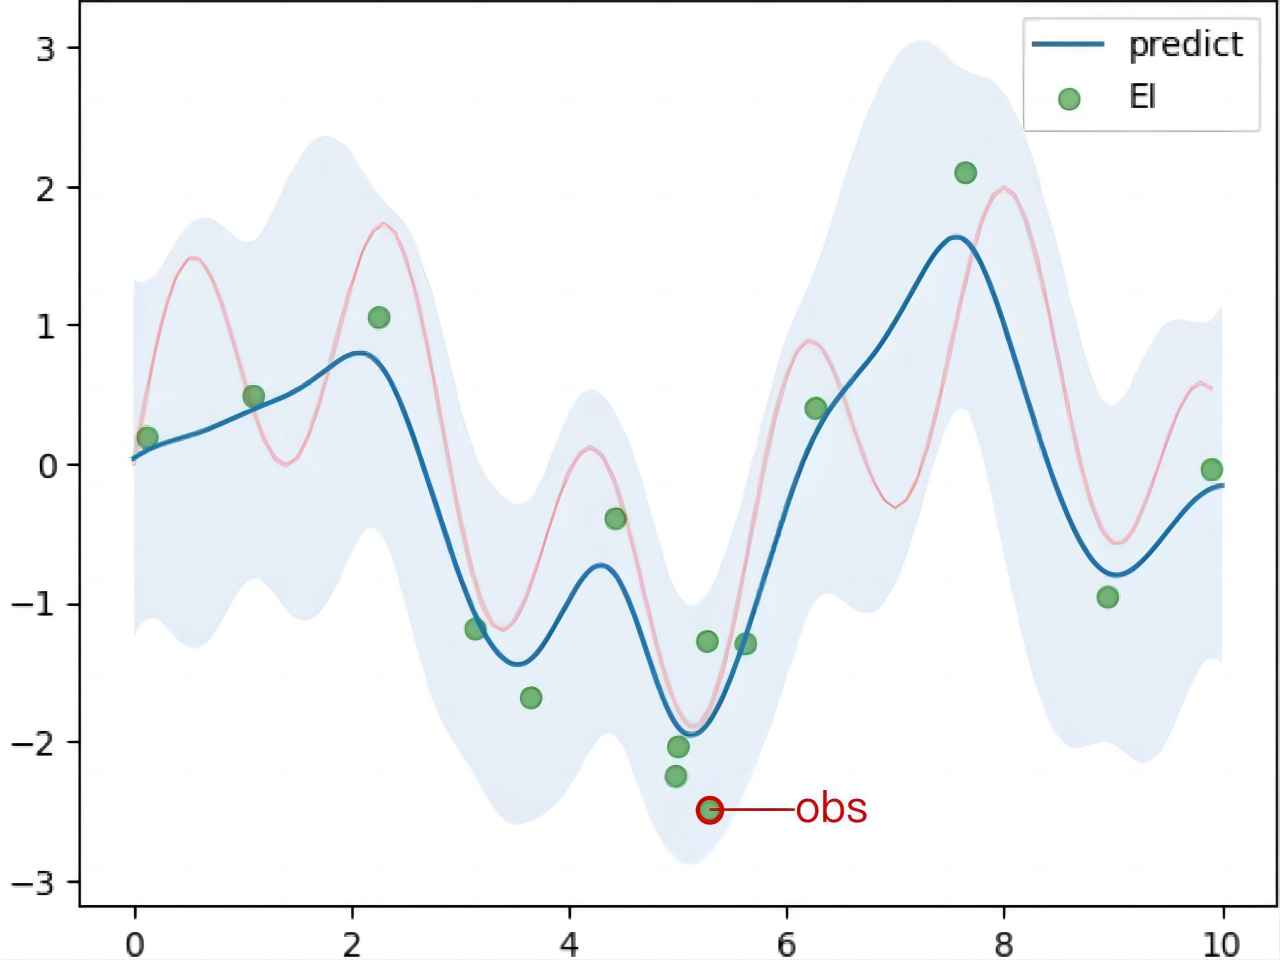
\includegraphics[width=1\textwidth]{D:/outputway/arXiv/figures/EI.jpg}
        \caption{Using EI for output method based on observation}
    \end{subfigure}
    \begin{subfigure}[t]{.48\linewidth}
        \centering
        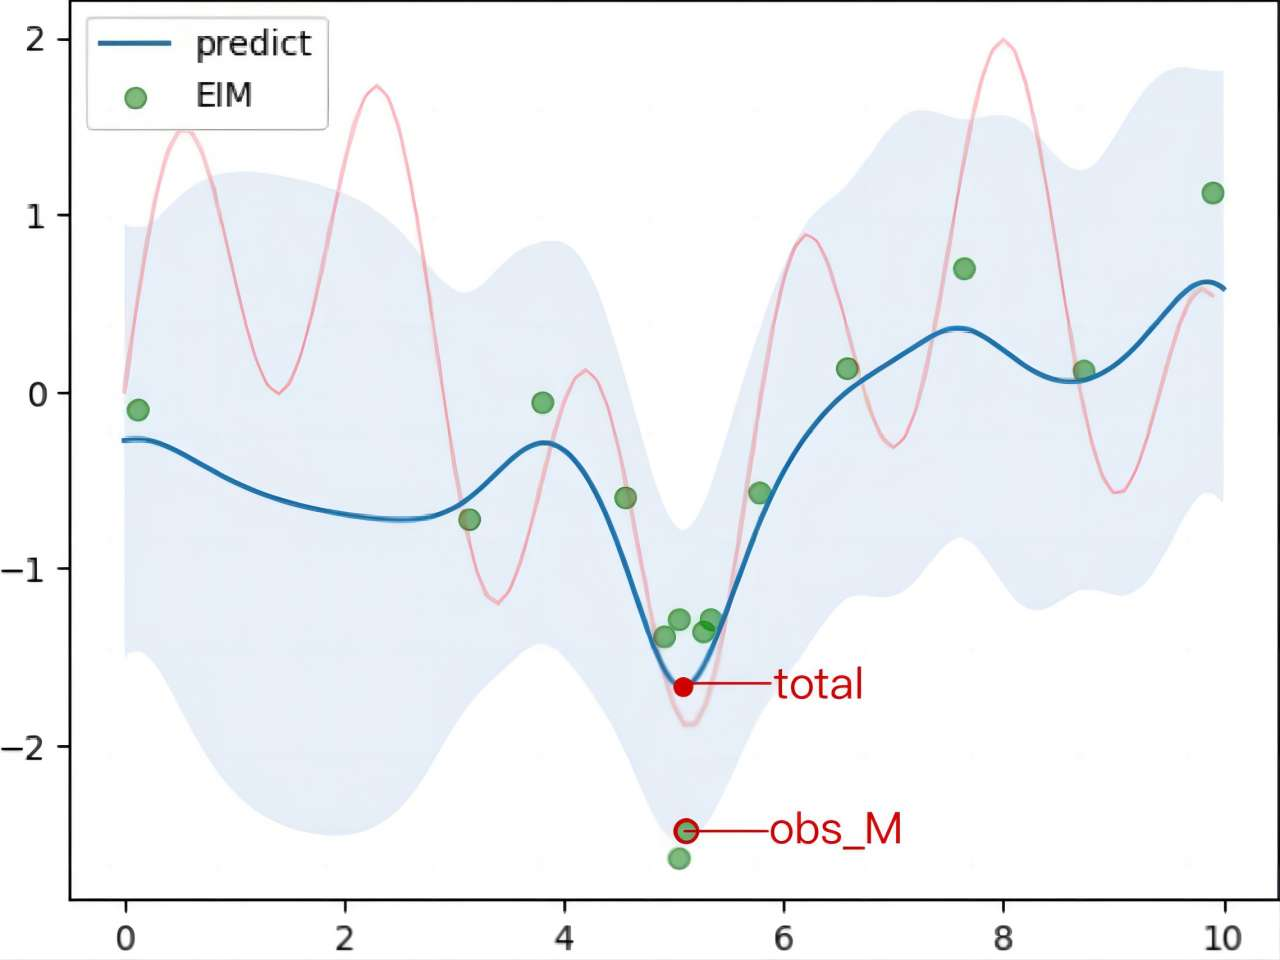
\includegraphics[width=1\textwidth]{D:/outputway/arXiv/figures/EIM.jpg}
        \caption{Using EIM for output method based on prediction}
    \end{subfigure}
    \caption{The above two figures show the results of Bayesian optimization for a one-dimensional noise function. The pale red curve is the true function curve, and the blue one is the curve of the predicted mean function of the GP. The green dot is the observation point selected by the acquisition function. The acquisition function used in the left figure is EI, which corresponds to the output method '\textbf{obs}', which will directly output the point corresponding to the smallest observation. The acquisition function for the right figure is EIM, which shows two outputs based on the predicted values. Method '\textbf{total}' corresponds to the minimum value of the predicted mean function (blue curve), and '\textbf{obs\_M}' is the point with the largest predicted mean (blue curve) corresponding to the coordinates of all observed points (green dots).}
    \label{Fig1}
\end{figure}




\section{Experimental results and analysis.}
  \subsection{Noise-free experimental results}
  \hspace{2em}We first focus on the experimental results for the noiseless problem. In the noise-free problem, the methods \textbf{obs},\textbf{obs\_M} are exactly the same since the observations of the observation points are all accurate. We only need to compare the \textbf{obs} and \textbf{total} methods and analyze whether the predictive output method can output better points as the final result. Of course, it makes sense to consider \textbf{obs} as the most reasonable output method under noise-free conditions. The main purpose of our noise-free experiments is to investigate the specific gap between the optimization efficiency of these two output methods under noise-free conditions. Table 2 details the specific differences between these two output methods:
  \begin{table}[!ht]
    \renewcommand{\arraystretch}{1.3}
    \centering
    \resizebox{1\columnwidth}{!}{
    \begin{tabular}{|c|ccc|c|ccc|}
    \hline
        2D & obs & total & total vs obs & 4D & obs & total & total vs obs \\ \hline
        F1 & 0.00\% & 0.00\% & 0.00\% & F1 & 0.00\% & 0.00\% & 0.00\% \\ 
        F2 & 5.71\% & 59.70\% & 50.71\% & F2 & 6589.66\% & 7861.45\% & 585.31\% \\ 
        F3 & 10.22\% & 27.81\% & 16.80\% & F3 & 26.95\% & 56.09\% & 23.06\% \\ 
        F4 & 5.01\% & 18.19\% & 12.62\% & F4 & 29.90\% & 63.32\% & 26.56\% \\ 
        F5 & 0.00\% & 0.00\% & 0.00\% & F5 & 0.00\% & 0.00\% & 0.00\% \\ 
		\cline{1-8}
        F6 & 1.52\% & 3.45\% & 1.89\% & F6 & 31.23\% & 105.48\% & 58.40\% \\ 
        F7 & 0.08\% & 0.18\% & 0.10\% & F7 & 0.05\% & 0.09\% & 0.05\% \\ 
        F8 & 0.07\% & 1.75\% & 1.68\% & F8 & 4.33\% & 5.16\% & 0.84\% \\ 
        F9 & 0.12\% & 3.66\% & 3.54\% & F9 & 5.76\% & 11.17\% & 5.25\% \\ 
		\cline{1-8}
        F10 & 15.30\% & 1282.36\% & 1133.40\% & F10 & 454.52\% & 4275.66\% & 1253.11\% \\ 
        F11 & 8.50\% & 719.52\% & 656.81\% & F11 & 22.84\% & 2774.84\% & 2255.78\% \\ 
        F12 & 1645.98\% & 2907234.96\% & 1209546.08\% & F12 & 526280.42\% & 27772809.81\% & 11673.63\% \\ 
        F13 & 0.96\% & 1.78\% & 0.81\% & F13 & 27.39\% & 12.98\% & -11.03\% \\ 
        F14 & 0.01\% & 0.02\% & 0.02\% & F14 & 0.01\% & 0.03\% & 0.01\% \\ 
		\cline{1-8}
        F15 & 5.26\% & 23.30\% & 17.33\% & F15 & 22.63\% & 64.67\% & 34.49\% \\ 
        F16 & 0.74\% & 26.55\% & 25.71\% & F16 & 3.20\% & 14.22\% & 10.55\% \\ 
        F17 & 0.52\% & 4.43\% & 3.89\% & F17 & 0.91\% & 1.20\% & 0.30\% \\ 
        F18 & 0.76\% & 11.46\% & 10.62\% & F18 & 2.40\% & 3.50\% & 1.08\% \\ 
        F19 & 0.25\% & 10.95\% & 10.68\% & F19 & 2.90\% & 14.37\% & 11.13\% \\ 
		\cline{1-8}
        F20 & 1.64\% & 5.11\% & 3.41\% & F20 & 2.78\% & 6.00\% & 3.13\% \\ 
        F21 & 0.07\% & 0.14\% & 0.07\% & F21 & 0.70\% & 0.84\% & 0.13\% \\ 
        F22 & 0.46\% & 0.75\% & 0.29\% & F22 & 3.62\% & 3.87\% & 0.24\% \\ 
        F23 & 4.48\% & 50.64\% & 44.24\% & F23 & 3.10\% & 24.36\% & 20.63\% \\ 
        F24 & 5.11\% & 27.33\% & 21.20\% & F24 & 20.30\% & 49.25\% & 24.22\% \\ \hline
    \end{tabular}
	}
	\caption{Noiseless results}
\end{table}

 
  \hspace{2em}The first two columns in the table are the loss rate of the output methods \textbf{obs},\textbf{obs\_M} relative to the global optimal value of each test function. The third columns is the relative loss rates of these two output methods. For two-dimensional problems, the predictive method \textbf{total} is significantly less efficient in optimization than \textbf{obs} when applied to the functions F2, F10, F11, and F12. A review of Table 1 reveals a common feature of these functions: their conditioning levels are significantly high, exceeding $10^6$. The standard deviation of each of these functions is very large, resulting in high noise levels. The high noise level can easily mask the original structural characteristics of the objective function, making it difficult to build a suitable model for the Gaussian process to predict. By examining Table 2, it can be seen that the loss rate of \textbf{obs} is likewise relatively high on these four functions compared to the others, which further suggests that the surrogate model struggles due to high conditioning levels. Therefore, it can be concluded that for noiseless problems, low accuracy in surrogate model modeling can greatly increase the loss rate of predictive output methods, in which case observational output method \textbf{obs} is more plausible. For simpler functions, the results in the third column show that the loss ratio of \textbf{total} relative to \textbf{obs} is mostly above $10\%$. For more complex functions such as F10, F12, etc., the gap between the optimization results will increase further. Therefore, for noise-free problems, we should indeed directly use the observation-based Bayesian optimization result output method (The loss rate of \textbf{total} relative to \textbf{obs} in all test functions is greater than 0). For 4D problems, the conclution remains same, however, after increasing the dimension, we find that the relative loss rate of these two output methods begins to decrease on many functions.This will be discussed later in the article.


  \subsection{Experimental results for the 2D noise problem}
  \hspace{2em}In the previous section, we briefly compared the optimization results of the observative and predictive outputs on 24 noise-free functions. In this section, we will pick out some functions and add noise to them as new optimization problems. In order to ensure the consistency of the conclusions, we will use EI as the acquisition function for the observable output method (\textbf{obs}), and EIM for the predictive output method (\textbf{obs\_M}, \textbf{total} ). It was noted that in the noisy problems, obs is no longer exactly the same as \textbf{obs\_M}, as the observed value will no longer be accurate.(See Section 3.2 for details on noise settings). We will use the Instant Regret as the vertical axis of the figures, and the number of iterations of BO as the horizontal axis to generate curves for analysis. For example, in each iteration of BO, EI selects a point as the next observation. We subtract the optimal value of the function from the value of the real function corresponding to the selected point to get the instantant regret value of EI at the corresponding round. EIM can do the same for a similar curve, and for comparison, we have added a curve corresponding to the acquisition function (denoted random) completely choose points randomly. For our three output methods (\textbf{obs},\textbf{obs\_M}, \textbf{total}), they will also choose a point as the output result of the round in each iteration of BO, so we can also obtain the instantant regret curves of the three methods in the same way for analysis and comparison.
  
\begin{figure}[H]
    \centering
    \begin{subfigure}[t]{.32\linewidth}
        \centering
        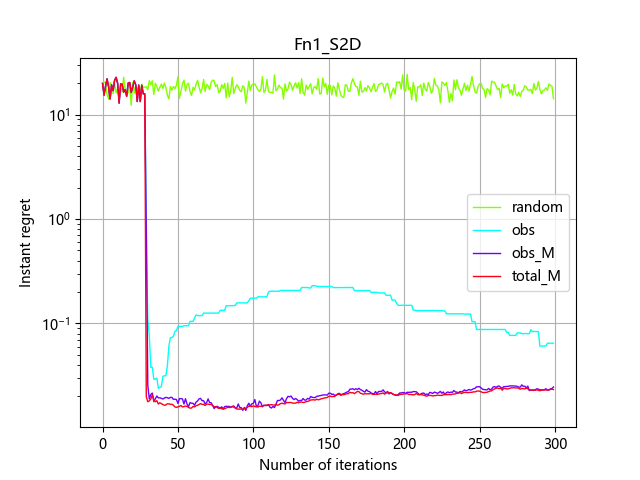
\includegraphics[width=1\textwidth]{D:/outputway/pictures/noise2D/S/Fn1_S2D_ins.png}
    \end{subfigure}
    \begin{subfigure}[t]{.32\linewidth}
        \centering
        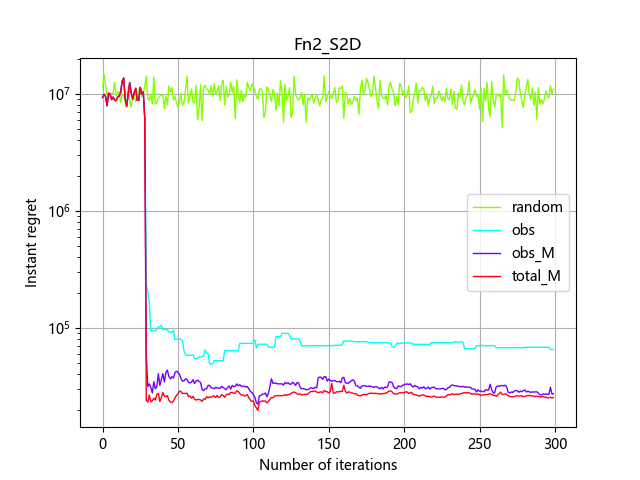
\includegraphics[width=1\textwidth]{D:/outputway/pictures/noise2D/S/Fn2_S2D_ins.png}
    \end{subfigure}
    \begin{subfigure}[t]{.32\linewidth}
        \centering
        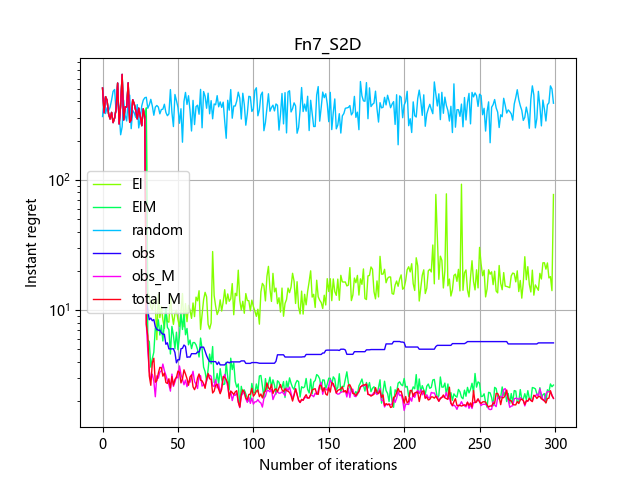
\includegraphics[width=1\textwidth]{D:/outputway/pictures/noise2D/S/Fn7_S2D_ins.png}
    \end{subfigure}
    \begin{subfigure}[t]{.32\linewidth}
        \centering
        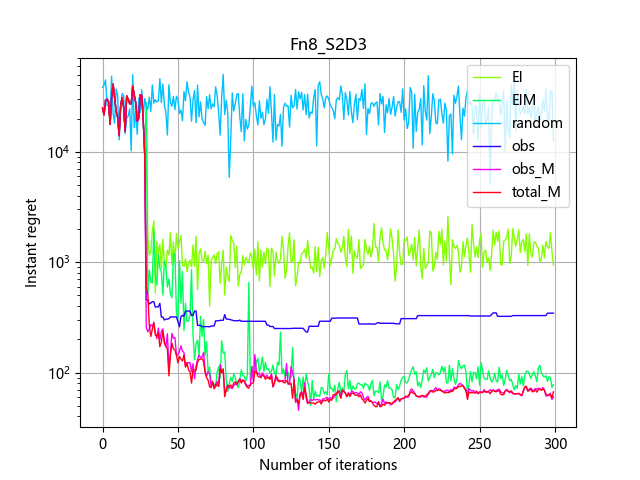
\includegraphics[width=1\textwidth]{D:/outputway/pictures/noise2D/S/Fn8_S2D_ins.png}
    \end{subfigure}
    \begin{subfigure}[t]{.32\linewidth}
        \centering
        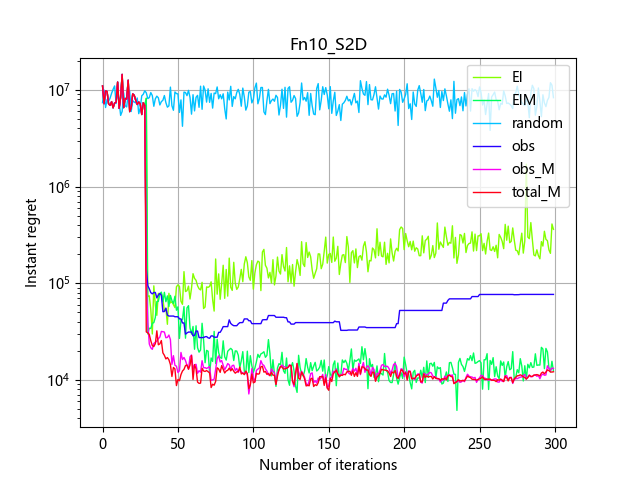
\includegraphics[width=1\textwidth]{D:/outputway/pictures/noise2D/S/Fn10_S2D_ins.png}
    \end{subfigure}
    \begin{subfigure}[t]{.32\linewidth}
        \centering
        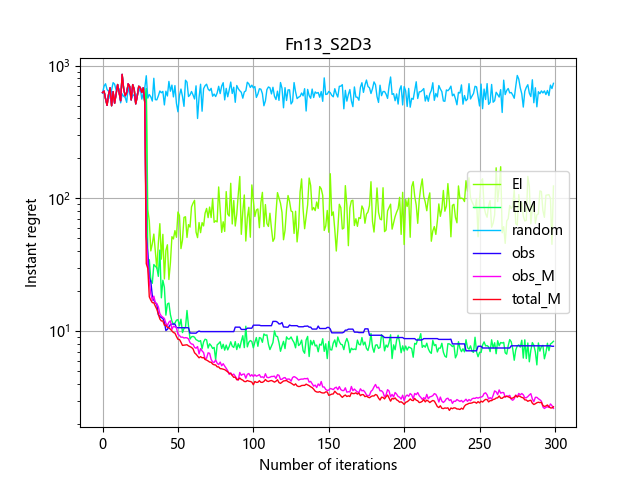
\includegraphics[width=1\textwidth]{D:/outputway/pictures/noise2D/S/Fn13_S2D_ins.png}
    \end{subfigure}
    \begin{subfigure}[t]{.32\linewidth}
        \centering
        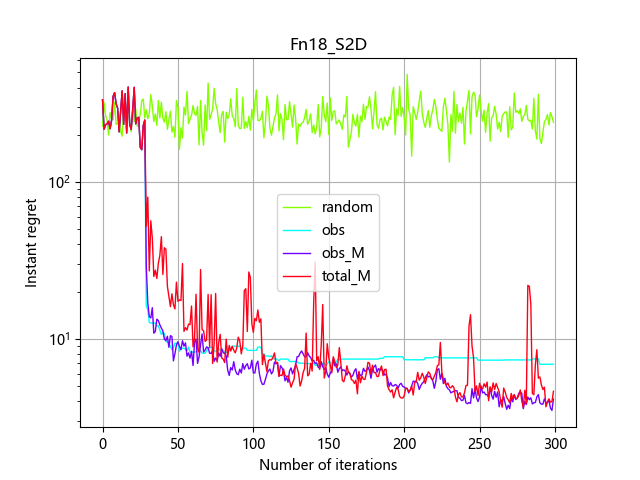
\includegraphics[width=1\textwidth]{D:/outputway/pictures/noise2D/S/Fn18_S2D_ins.png}
    \end{subfigure}
    \begin{subfigure}[t]{.32\linewidth}
        \centering
        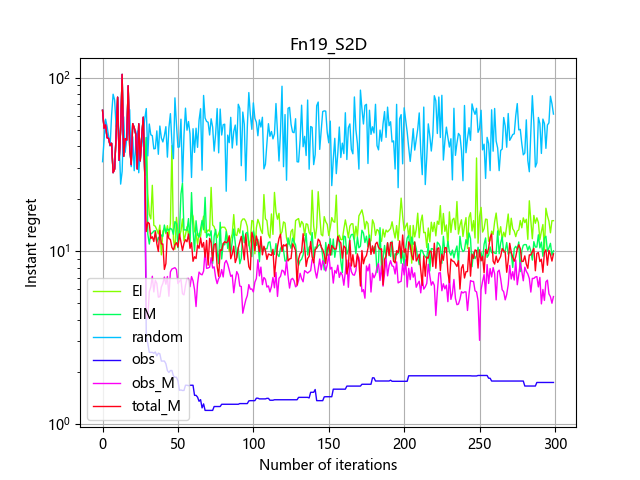
\includegraphics[width=1\textwidth]{D:/outputway/pictures/noise2D/S/Fn19_S2D_ins.png}
    \end{subfigure}
    \begin{subfigure}[t]{.32\linewidth}
        \centering
        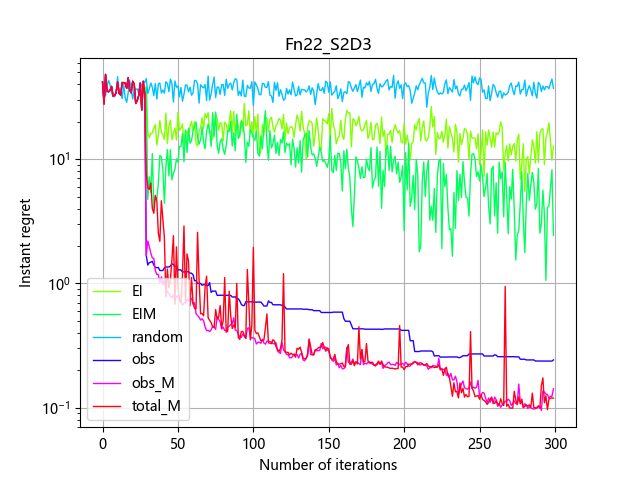
\includegraphics[width=1\textwidth]{D:/outputway/pictures/noise2D/S/Fn22_S2D_ins.png}
    \end{subfigure}
    \caption{2D optimization results(small noise)}
    \label{Fig2}
\end{figure}

\hspace{2em}It should be noted that the points found by the three acquisition functions(EI, EIM, random) described above at each iteration are used as the observation points of BO at the corresponding rounds, while the points found by the three output methods(\textbf{obs}, \textbf{obs\_M}, \textbf{total}) at each iteration are used as the output results of BO at the corresponding rounds. The meaning of these two is essentially different. We draw the curves of the three acquisition functions mainly to observe the difference of the point selection strategies of the three acquisition functions in different optimization problems; while the real interest of this paper is the difference of the three output methods, and the curves of the three acquisition functions are not the main research object. 

\hspace{2em}In the two-dimensional small noise optimization result figures, we can see that the curve of EI is always above the curve of EIM, which essentially reflects the difference between the two acquisition functions in terms of point selection strategy: EI is more inclined to explore and EIM is more inclined to development. There is no superiority or disadvantage between these two strategies, for different optimization problems they will have different optimization results. For the three output methods, since we all choose the output point after the budget is exhausted as the final output result, we can directly judge the quality of their output results by observing the average regret corresponding to the end of the curve.

\hspace{2em}Let's start with two predictive output methods. From Figure2, there is little difference between \textbf{obs\_M} and \textbf{total} in the final optimization results, but the output of \textbf{total} shows great instability in some functions. For example, for the function Fn18, the output of \textbf{total} in turns 280-290 fluctuates greatly. Considering that our budget is actually arbitrary, if the budget happens to be between 280-290, the final output returned by \textbf{total} will be very bad. Compared with \textbf{total}, the output value of \textbf{obs\_M} is more stable, so for two-dimensional problems with small noise, we recommend using \textbf{obs\_M}instead of \textbf{total} if you want to use a predictive output method.

\begin{figure}[H]
    \centering
    \begin{subfigure}[t]{.32\linewidth}
        \centering
        \includegraphics[width=1\textwidth]{D:/outputway/pictures/noise2D/M/Fn1_M2D_ins.png}
    \end{subfigure}
    \begin{subfigure}[t]{.32\linewidth}
        \centering
        \includegraphics[width=1\textwidth]{D:/outputway/pictures/noise2D/M/Fn2_M2D_ins.png}
    \end{subfigure}
    \begin{subfigure}[t]{.32\linewidth}
        \centering
        \includegraphics[width=1\textwidth]{D:/outputway/pictures/noise2D/M/Fn7_M2D_ins.png}
    \end{subfigure}
    \begin{subfigure}[t]{.32\linewidth}
        \centering
        \includegraphics[width=1\textwidth]{D:/outputway/pictures/noise2D/M/Fn8_M2D_ins.png}
    \end{subfigure}
    \begin{subfigure}[t]{.32\linewidth}
        \centering
        \includegraphics[width=1\textwidth]{D:/outputway/pictures/noise2D/M/Fn10_M2D_ins.png}
    \end{subfigure}
    \begin{subfigure}[t]{.32\linewidth}
        \centering
        \includegraphics[width=1\textwidth]{D:/outputway/pictures/noise2D/M/Fn13_M2D_ins.png}
    \end{subfigure}
    \begin{subfigure}[t]{.32\linewidth}
        \centering
        \includegraphics[width=1\textwidth]{D:/outputway/pictures/noise2D/M/Fn18_M2D_ins.png}
    \end{subfigure}
    \begin{subfigure}[t]{.32\linewidth}
        \centering
        \includegraphics[width=1\textwidth]{D:/outputway/pictures/noise2D/M/Fn19_M2D_ins.png}
    \end{subfigure}
    \begin{subfigure}[t]{.32\linewidth}
        \centering
        \includegraphics[width=1\textwidth]{D:/outputway/pictures/noise2D/M/Fn22_M2D_ins.png}
    \end{subfigure}
    \caption{2D optimization results(Medium noise)}
    \label{Fig3}
\end{figure}

\hspace{2em}As for the observative output method obs, we can see from Figure2 that the final output result of obs is much worse than \textbf{obs\_M} on most of the test functions, and its curve will always be above the curve of \textbf{obs\_M} after fewer rounds of iterations. This means that for any arbitrary given budget, the final output of obs is worse than \textbf{obs\_M}. However, in terms of optimization of the test function Fn19 , we find that obs has a clear advantage over other output methods. Further observation of the image corresponding to Fn19 reveals that the curves of EI, EIM, \textbf{obs\_M}, and  \textbf{total} are basically clustered at the same height, which actually indicates that the GP model models the function 19 poorly, the exploitation ability of the acquisition function is weak, and the prediction accuracy of the model is low. In this case, the results of the predictive output method are unreliable. Therefore, predictive output should be used with caution for highly complex problems with low modeling accuracy like Function 19. For general noise problems with good modeling accuracy, it is more reasonable to use predictive output methods (\textbf{obs\_M}). 

\hspace{2em}Figure3 illustrates the optimization results for moderate noise levels. It can be seen that with increased noise, the gap between the observational output method \textbf{obs} and the predictive output method widens further for most of the test functions. Overall, the conclusions for the choice of output methods are generally consistent with those under small noise.That is, for most problems with small noise, the use of the \textbf{obs\_M} output method is the best choice. The use of \textbf{obs} only needs to be considered if one is convinced that BO's surrogate has low predict accuracy, but in fact replacing the model may be the better choice in such cases. If we increase the noise level further (see Appendix B for details), the above conclusions still hold true, and when noise level is too high, the advantage of \textbf{obs} in Fn19 even no longer exists.

\subsection{Experimental results for the 4D noise problem}

\begin{figure}[H]
    \centering
    \begin{subfigure}[t]{.32\linewidth}
        \centering
        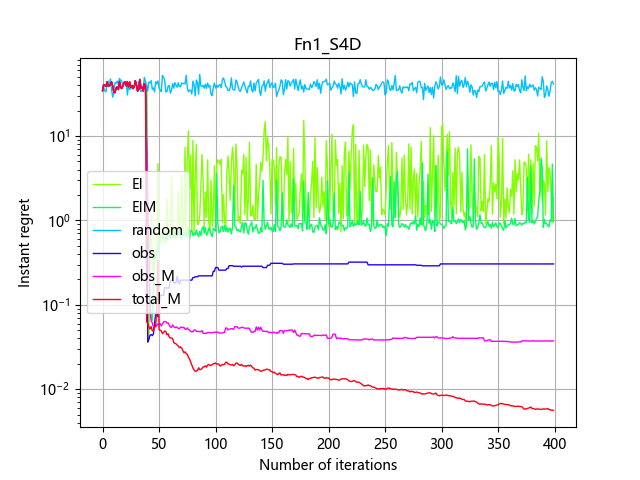
\includegraphics[width=1\textwidth]{D:/outputway/pictures/noise4D/S/Fn1_S4D_ins.png}
    \end{subfigure}
    \begin{subfigure}[t]{.32\linewidth}
        \centering
        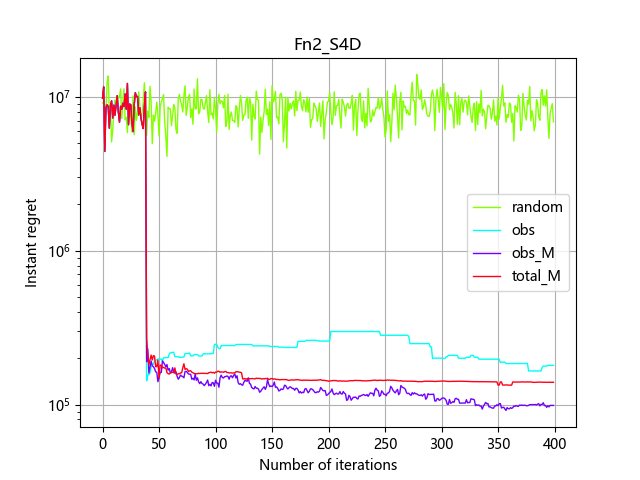
\includegraphics[width=1\textwidth]{D:/outputway/pictures/noise4D/S/Fn2_S4D_ins.png}
    \end{subfigure}
    \begin{subfigure}[t]{.32\linewidth}
        \centering
        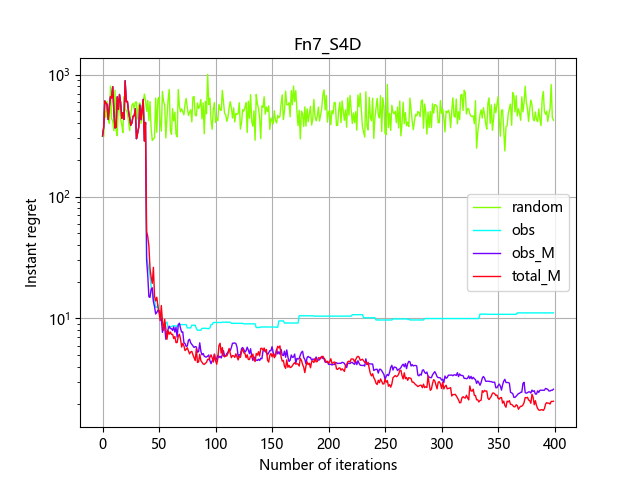
\includegraphics[width=1\textwidth]{D:/outputway/pictures/noise4D/S/Fn7_S4D_ins.png}
    \end{subfigure}
    \begin{subfigure}[t]{.32\linewidth}
        \centering
        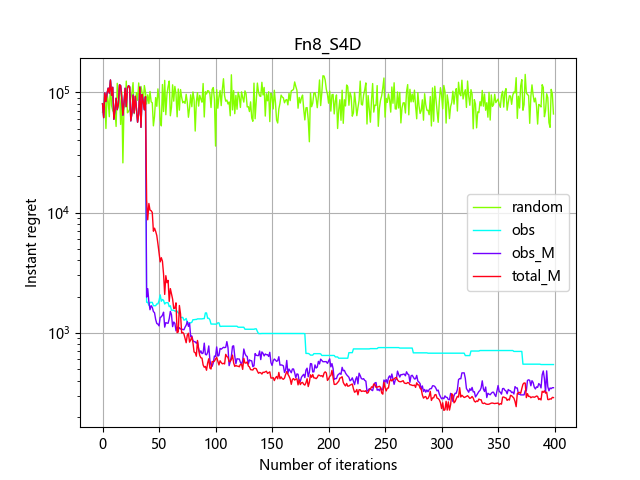
\includegraphics[width=1\textwidth]{D:/outputway/pictures/noise4D/S/Fn8_S4D_ins.png}
    \end{subfigure}
    \begin{subfigure}[t]{.32\linewidth}
        \centering
        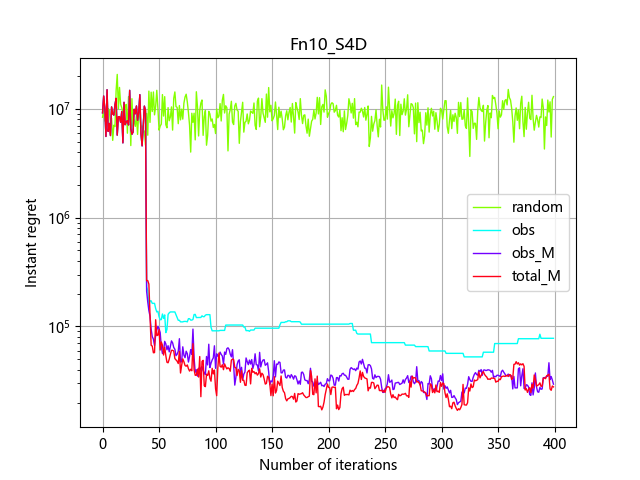
\includegraphics[width=1\textwidth]{D:/outputway/pictures/noise4D/S/Fn10_S4D_ins.png}
    \end{subfigure}
    \begin{subfigure}[t]{.32\linewidth}
        \centering
        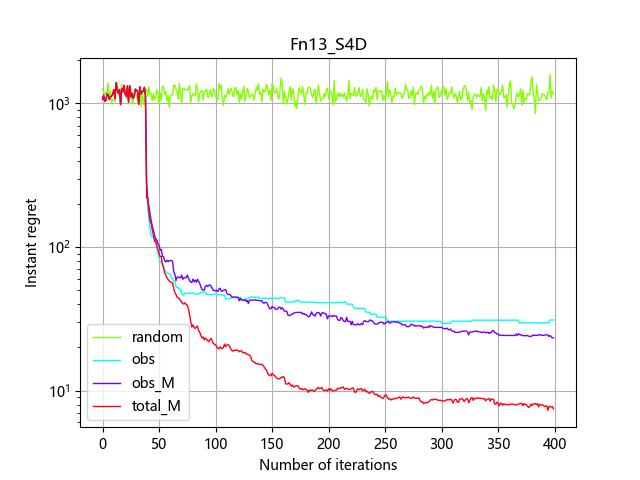
\includegraphics[width=1\textwidth]{D:/outputway/pictures/noise4D/S/Fn13_S4D_ins.png}
    \end{subfigure}
    \begin{subfigure}[t]{.32\linewidth}
        \centering
        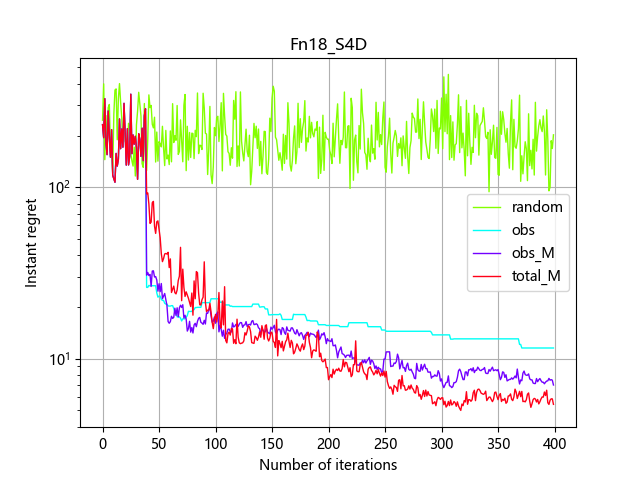
\includegraphics[width=1\textwidth]{D:/outputway/pictures/noise4D/S/Fn18_S4D_ins.png}
    \end{subfigure}
    \begin{subfigure}[t]{.32\linewidth}
        \centering
        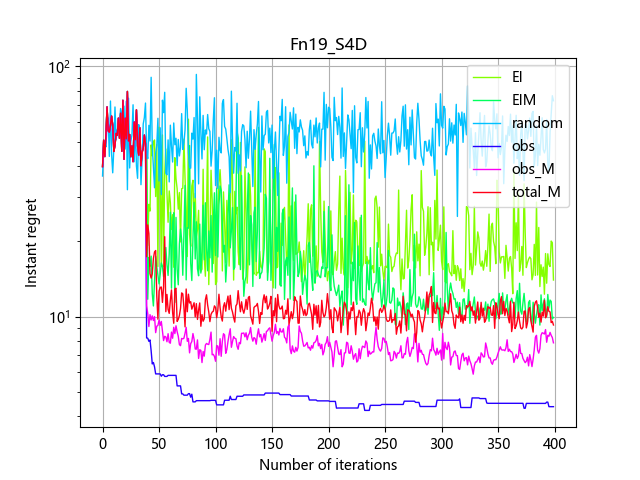
\includegraphics[width=1\textwidth]{D:/outputway/pictures/noise4D/S/Fn19_S4D_ins.png}
    \end{subfigure}
    \begin{subfigure}[t]{.32\linewidth}
        \centering
        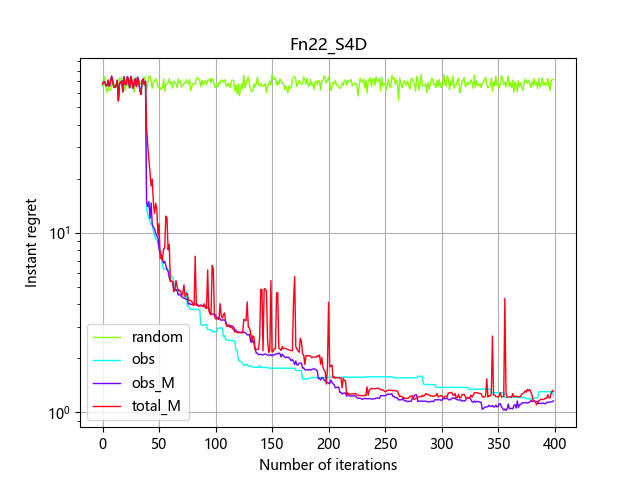
\includegraphics[width=1\textwidth]{D:/outputway/pictures/noise4D/S/Fn22_S4D_ins.png}
    \end{subfigure}
    \caption{4D optimization results(small noise)}
    \label{Fig4}
\end{figure}

\hspace{2em}In this section we increase the dimensionality of the optimisation problem from 2 to 4, which will allow the search space to expand geometrically. Figure 4 shows the optimisation results on a low noise level problem. Compared to the 2-dimensional image, we can clearly notice that the output method \textbf{total} starts to become competitive. For example, on the function Fn1, which is the simplest form and the least difficult to optimise, textbf{total} outputs far better results than the other output methods. The same is true on function Fn13. There is also a small advantage over \textbf{obs\_M} on functions Fn7 and Fn18. This is mainly due to the fact that \textbf{obs\_M} can only select among the points that have been observed, and even though we have increased the maximum number of iterations to 400 for the four-dimensional problem, 400 points is still too few for a four-dimensional search space. And, as we discussed earlier, both for EI and EIM, these acquisition functions selected points are not used exclusively for exploitation; they are also required to undertake certain exploration tasks. This leads to a further reduction in the proportion of these 400 points that contain higher points. In the case of \textbf{total}, on the other hand, the 400 points it selects are fully focused on exploitation and are not limited to observed points. This makes it more likely to find local optimal value points. Whereas for higher dimensional problems, too large a search space can make it extremely difficult to find the global optimal solution, in which case finding the local optimal solution may instead be a better choice. However, it is worth noting that raising the dimensionality does not solve the problem of the instability of \textbf{total} output results. For example, on Fn22 \textbf{total} still has large fluctuations, which means that it is still possible that it may give an extremely bad point as an optimisation result for output in a particular experiment. There is no denying that \textbf{total} is competitive in slightly higher dimensional optimisation problems, but choosing it still carries the risk of instability. Therefore, we take a conservative view on the use of \textbf{total}, i.e., it should be used with caution. In contrast, the performance of \textbf{obs\_M} remains relatively stable. It outperforms \textbf{obs} on all test problems except Fn19, and is not significantly weaker or even better than \textbf{total} on most problems. Taken together, \textbf{obs\_M} continues to be the most reasonable choice in 4 dimensions with low noise levels. We similarly tried to continue to increase the noise level (see Appendix B for details) and the conclusions obtained remains the same.

\section{Conclusion}

\hspace{2em}In the previous section we conducted numerical experiments on optimisation test problems without noise and with different noise levels and dimensions. The main conclusions are summarised as follows: 


\begin{itemize}[itemsep=2pt,topsep=0pt,parsep=0pt]
    \item[$\bullet$] For the noiseless problem, directly using the observation-based output \textbf{obs} is the most reasonable choice. 
    \item[$\bullet$] For the noisy problem, using the predictive-based output is superior to the observation-based output in most of the cases, even when the noise level is low.Considering that the output results of \textbf{total} are not stable, the use of \textbf{obs\_M} is the most reasonable choice.
    \item[$\bullet$] For more complex problems, when the prediction accuracy of BO's surrogate model is low, the predictive-based output method should be used with caution. This is because the model's prediction of the objective function is less credible. In this case, the choice of observation-based output will often give better output results, but in practice it is meaningless. If we can be sure that the model is less predictive, then we should consider replacing the model rather than discussing what output to use.
    \item[$\bullet$] When the optimisation problem is of high dimensionality, the use of \textbf{total} can be considered, but it still carries the risk of unstable output results.  
       
    \end{itemize} 

\hspace{2em}It is also worth mentioning that the form of the noise can likewise influence the choice of output methods. Our experiments above only discuss homogeneous noise, and the conclusions may change when the noise becomes non-homogeneous. We briefly discuss this scenario in Appendix A and give the corresponding experimental results.



\clearpage

\bibliographystyle{unsrtnat}
\bibliography{references}  %%% Uncomment this line and comment out the ``thebibliography'' section below to use the external .bib file (using bibtex) .


%%% Uncomment this section and comment out the \bibliography{references} line above to use inline references.
% \begin{thebibliography}{1}

% 	\bibitem{kour2014real}
% 	George Kour and Raid Saabne.
% 	\newblock Real-time segmentation of on-line handwritten arabic script.
% 	\newblock In {\em Frontiers in Handwriting Recognition (ICFHR), 2014 14th
% 			International Conference on}, pages 417--422. IEEE, 2014.

% 	\bibitem{kour2014fast}
% 	George Kour and Raid Saabne.
% 	\newblock Fast classification of handwritten on-line arabic characters.
% 	\newblock In {\em Soft Computing and Pattern Recognition (SoCPaR), 2014 6th
% 			International Conference of}, pages 312--318. IEEE, 2014.

% 	\bibitem{hadash2018estimate}
% 	Guy Hadash, Einat Kermany, Boaz Carmeli, Ofer Lavi, George Kour, and Alon
% 	Jacovi.
% 	\newblock Estimate and replace: A novel approach to integrating deep neural
% 	networks with existing applications.
% 	\newblock {\em arXiv preprint arXiv:1804.09028}, 2018.

% \end{thebibliography}

\clearpage

{\centering\section*{Appendix}}
\appendix
\section{Non-homogeneous noise experimental results}
\subsection{2-dimensional experiments}
The basic settings of the experiments are the same as those in 4.2, with the only difference being that the noise settings are no longer homogeneous variance, but are set as follows:
\begin{equation}\label{eq11}
	f_{GN}(f,\beta) = f \times exp(\beta\mathcal{N}(0,1)) 
\end{equation}
where $mathcal{N}(0,1)$ represents random sampling from the standard normal distribution, and $beta$ is the parameter that controls the magnitude of the noise, here we set it to 0.1. Note that the value of noise here will be related to the true value of the function. Also similar to 4.2, we give the following image of the experimental results:

\begin{figure}[H]
    \centering
    \begin{subfigure}[t]{.32\linewidth}
        \centering
        \includegraphics[width=1\textwidth]{D:/outputway/pictures/noise2D_old_EIM/Fn1_M2D_ins.png}
    \end{subfigure}
    \begin{subfigure}[t]{.32\linewidth}
        \centering
        \includegraphics[width=1\textwidth]{D:/outputway/pictures/noise2D_old_EIM/Fn2_M2D_ins.png}
    \end{subfigure}
    \begin{subfigure}[t]{.32\linewidth}
        \centering
        \includegraphics[width=1\textwidth]{D:/outputway/pictures/noise2D_old_EIM/Fn7_M2D_ins.png}
    \end{subfigure}
    \begin{subfigure}[t]{.32\linewidth}
        \centering
        \includegraphics[width=1\textwidth]{D:/outputway/pictures/noise2D_old_EIM/Fn8_M2D_ins.png}
    \end{subfigure}
    \begin{subfigure}[t]{.32\linewidth}
        \centering
        \includegraphics[width=1\textwidth]{D:/outputway/pictures/noise2D_old_EIM/Fn10_M2D_ins.png}
    \end{subfigure}
    \begin{subfigure}[t]{.32\linewidth}
        \centering
        \includegraphics[width=1\textwidth]{D:/outputway/pictures/noise2D_old_EIM/Fn13_M2D_ins.png}
    \end{subfigure}
    \begin{subfigure}[t]{.32\linewidth}
        \centering
        \includegraphics[width=1\textwidth]{D:/outputway/pictures/noise2D_old_EIM/Fn18_M2D_ins.png}
    \end{subfigure}
    \begin{subfigure}[t]{.32\linewidth}
        \centering
        \includegraphics[width=1\textwidth]{D:/outputway/pictures/noise2D_old_EIM/Fn19_M2D_ins.png}
    \end{subfigure}
    \begin{subfigure}[t]{.32\linewidth}
        \centering
        \includegraphics[width=1\textwidth]{D:/outputway/pictures/noise2D_old_EIM/Fn22_M2D_ins.png}
    \end{subfigure}
    \caption{2D optimization results(Non-homogeneous noise)}
    \label{Fig5}
\end{figure}
The results reflected in the figures are basically similar to those in 4.2, with the only difference being that for functions with large standard deviations (e.g. Fn2, Fn10), the observative output methods in non-homogeneous noise is much better than the predictive output method. This is because when the noise value is positively correlated with the true value of the function, the point with the smaller value of the function corresponds to the less noise, so if we observe that the value of a point is small, it is most likely because the function value corresponding to that point is also small, rather than due to extreme noise. In this case, the observant output method is more reliable than the predictive output methods, even if noise is affected.

\subsection{4-dimensional experiments}
Keeping the other settings unchanged, now we increase the dimension of the test function to 4 dimensions (the number of initial points and the total budget are increased to 40 and 400 respectively), and we get the following result:

 \begin{figure}[ht]
    \centering
    \begin{subfigure}[t]{.32\linewidth}
        \centering
        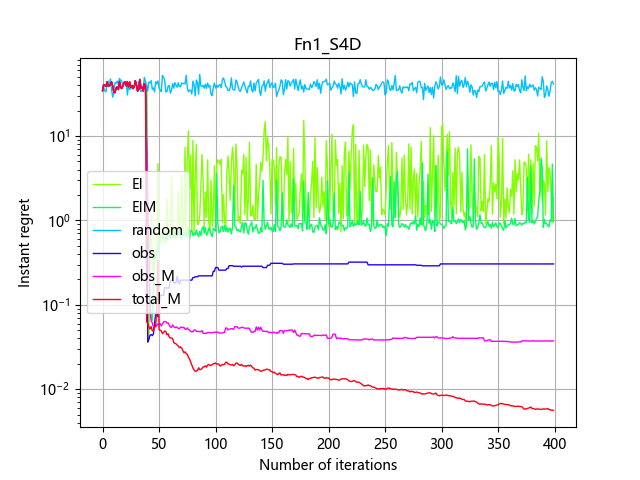
\includegraphics[width=1\textwidth]{D:/outputway/pictures/noise4D/S/Fn1_S4D_ins.png}
    \end{subfigure}
    \begin{subfigure}[t]{.32\linewidth}
        \centering
        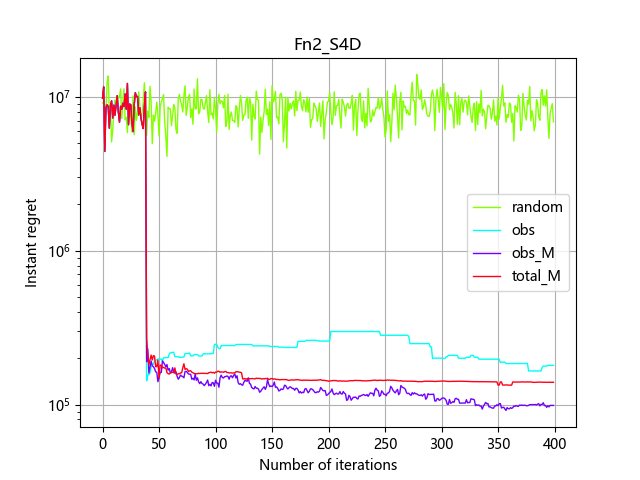
\includegraphics[width=1\textwidth]{D:/outputway/pictures/noise4D/S/Fn2_S4D_ins.png}
    \end{subfigure}
    \begin{subfigure}[t]{.32\linewidth}
        \centering
        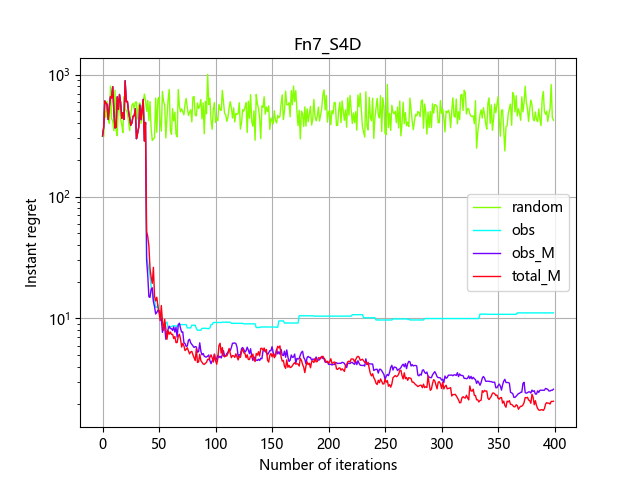
\includegraphics[width=1\textwidth]{D:/outputway/pictures/noise4D/S/Fn7_S4D_ins.png}
    \end{subfigure}
    \begin{subfigure}[t]{.32\linewidth}
        \centering
        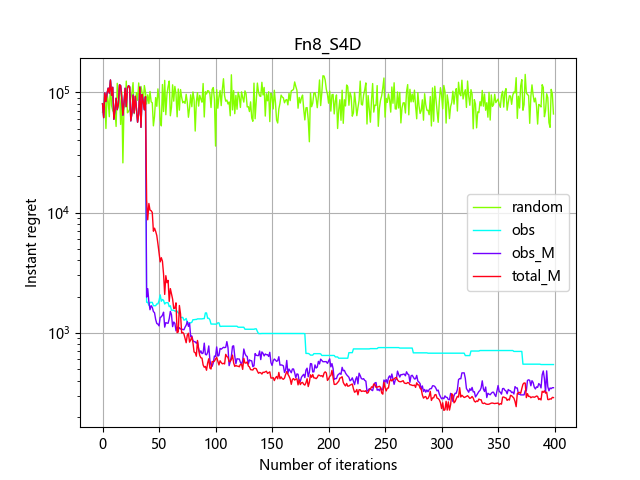
\includegraphics[width=1\textwidth]{D:/outputway/pictures/noise4D/S/Fn8_S4D_ins.png}
    \end{subfigure}
    \begin{subfigure}[t]{.32\linewidth}
        \centering
        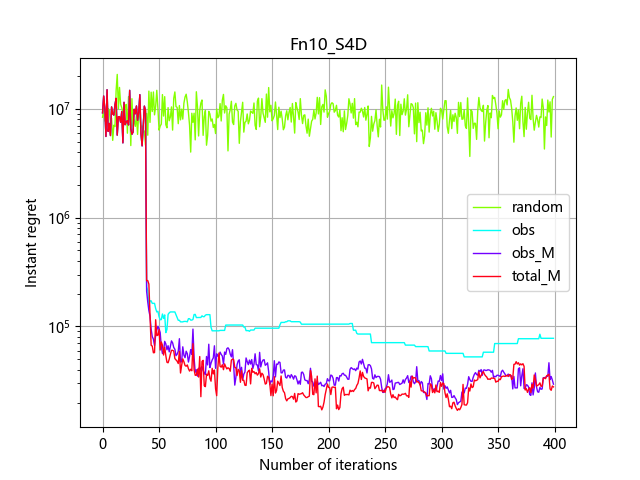
\includegraphics[width=1\textwidth]{D:/outputway/pictures/noise4D/S/Fn10_S4D_ins.png}
    \end{subfigure}
    \begin{subfigure}[t]{.32\linewidth}
        \centering
        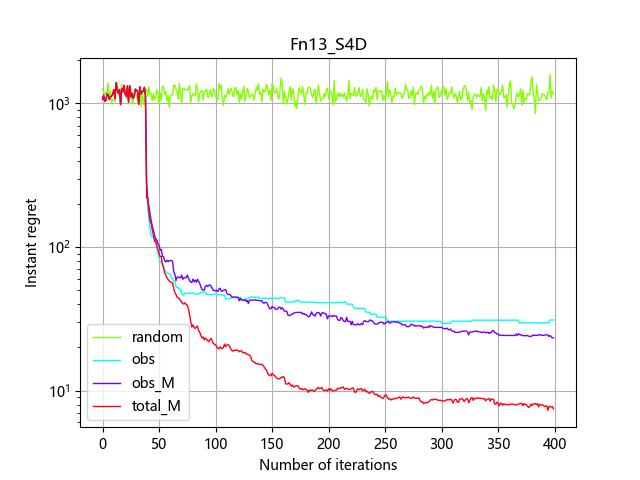
\includegraphics[width=1\textwidth]{D:/outputway/pictures/noise4D/S/Fn13_S4D_ins.png}
    \end{subfigure}
    \begin{subfigure}[t]{.32\linewidth}
        \centering
        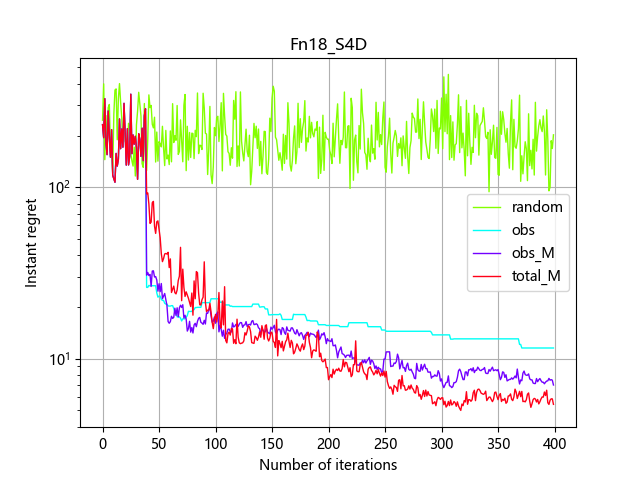
\includegraphics[width=1\textwidth]{D:/outputway/pictures/noise4D/S/Fn18_S4D_ins.png}
    \end{subfigure}
    \begin{subfigure}[t]{.32\linewidth}
        \centering
        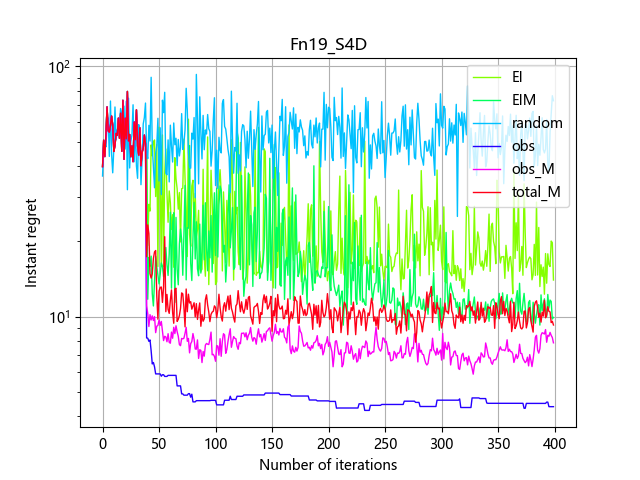
\includegraphics[width=1\textwidth]{D:/outputway/pictures/noise4D/S/Fn19_S4D_ins.png}
    \end{subfigure}
    \begin{subfigure}[t]{.32\linewidth}
        \centering
        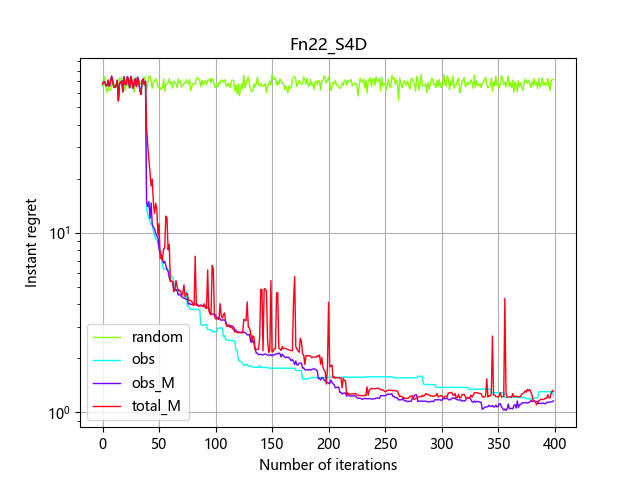
\includegraphics[width=1\textwidth]{D:/outputway/pictures/noise4D/S/Fn22_S4D_ins.png}
    \end{subfigure}
    \caption{4D optimization results(homogeneous noise)}
    \label{Fig6}
\end{figure}
From the 4D image, we can draw conclusions that are basically the same as those of 2D. We noticed that after the dimension increased, total began to show a certain competitiveness compared with the other two output methods, especially in the simplest test function, Fn1, which was significantly ahead of the other two output methods. The characteristic of total is that it is a completely exploitation output method, although obs\_M also output the maximum value of prediction mean, but its output is limited to the observations selected by the acquisition function EI. As we mentioned earlier, EI is an exploratory algorithm, and the size of the search space increases dramatically when the dimension is increased to 4D, so that the benefits of exploration in a limited budget may be much lower than that of exploitation. However, there is still some instability in the output result of total (for example, Fn18), and the final result is not significantly better than obs\_M in most test functions, so we still do not recommend using the total output method under four-dimensional conditions.

\section{Other homogeneous noise experimental results}
\subsection{2-dimensional experiments}
\begin{figure}[H]
    \centering
    \begin{subfigure}[t]{.32\linewidth}
        \centering
        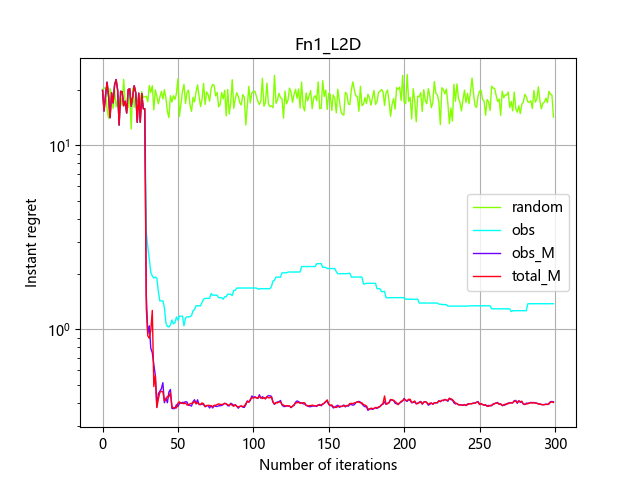
\includegraphics[width=1\textwidth]{D:/outputway/pictures/noise2D/L/Fn1_L2D_ins.png}
    \end{subfigure}
    \begin{subfigure}[t]{.32\linewidth}
        \centering
        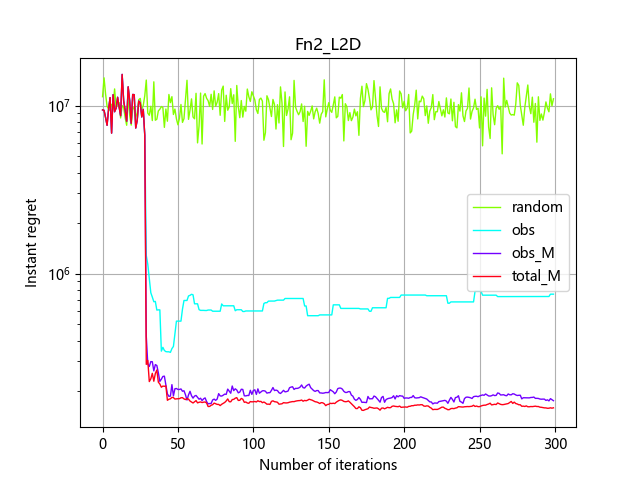
\includegraphics[width=1\textwidth]{D:/outputway/pictures/noise2D/L/Fn2_L2D_ins.png}
    \end{subfigure}
    \begin{subfigure}[t]{.32\linewidth}
        \centering
        \includegraphics[width=1\textwidth]{D:/outputway/pictures/noise2D/L/Fn7_L2D_ins.png}
    \end{subfigure}
    \begin{subfigure}[t]{.32\linewidth}
        \centering
        \includegraphics[width=1\textwidth]{D:/outputway/pictures/noise2D/L/Fn8_L2D_ins.png}
    \end{subfigure}
    \begin{subfigure}[t]{.32\linewidth}
        \centering
        \includegraphics[width=1\textwidth]{D:/outputway/pictures/noise2D/L/Fn10_L2D_ins.png}
    \end{subfigure}
    \begin{subfigure}[t]{.32\linewidth}
        \centering
        \includegraphics[width=1\textwidth]{D:/outputway/pictures/noise2D/L/Fn13_L2D_ins.png}
    \end{subfigure}
    \begin{subfigure}[t]{.32\linewidth}
        \centering
        \includegraphics[width=1\textwidth]{D:/outputway/pictures/noise2D/L/Fn18_L2D_ins.png}
    \end{subfigure}
    \begin{subfigure}[t]{.32\linewidth}
        \centering
        \includegraphics[width=1\textwidth]{D:/outputway/pictures/noise2D/L/Fn19_L2D_ins.png}
    \end{subfigure}
    \begin{subfigure}[t]{.32\linewidth}
        \centering
        \includegraphics[width=1\textwidth]{D:/outputway/pictures/noise2D/L/Fn22_L2D_ins.png}
    \end{subfigure}
    \caption{2D optimization results(Large noise)}
    \label{Fig7}
\end{figure}

\subsection{4-dimensional experiments}

\begin{figure}[H]
    \centering
    \begin{subfigure}[t]{.32\linewidth}
        \centering
        \includegraphics[width=1\textwidth]{D:/outputway/pictures/noise4D/M/Fn1_M4D_ins.png}
    \end{subfigure}
    \begin{subfigure}[t]{.32\linewidth}
        \centering
        \includegraphics[width=1\textwidth]{D:/outputway/pictures/noise4D/M/Fn2_M4D_ins.png}
    \end{subfigure}
    \begin{subfigure}[t]{.32\linewidth}
        \centering
        \includegraphics[width=1\textwidth]{D:/outputway/pictures/noise4D/M/Fn7_M4D_ins.png}
    \end{subfigure}
    \begin{subfigure}[t]{.32\linewidth}
        \centering
        \includegraphics[width=1\textwidth]{D:/outputway/pictures/noise4D/M/Fn8_M4D_ins.png}
    \end{subfigure}
    \begin{subfigure}[t]{.32\linewidth}
        \centering
        \includegraphics[width=1\textwidth]{D:/outputway/pictures/noise4D/M/Fn10_M4D_ins.png}
    \end{subfigure}
    \begin{subfigure}[t]{.32\linewidth}
        \centering
        \includegraphics[width=1\textwidth]{D:/outputway/pictures/noise4D/M/Fn13_M4D_ins.png}
    \end{subfigure}
    \begin{subfigure}[t]{.32\linewidth}
        \centering
        \includegraphics[width=1\textwidth]{D:/outputway/pictures/noise4D/M/Fn18_M4D_ins.png}
    \end{subfigure}
    \begin{subfigure}[t]{.32\linewidth}
        \centering
        \includegraphics[width=1\textwidth]{D:/outputway/pictures/noise4D/M/Fn19_M4D_ins.png}
    \end{subfigure}
    \begin{subfigure}[t]{.32\linewidth}
        \centering
        \includegraphics[width=1\textwidth]{D:/outputway/pictures/noise4D/M/Fn22_M4D_ins.png}
    \end{subfigure}
    \caption{4D optimization results(Medium noise)}
    \label{Fig8}
\end{figure}
\end{document}

